\documentclass[12pt, a4paper]{article}
%%import package named hightest
\usepackage{hightest}
\usepackage[export]{adjustbox}
\usepackage{wrapfig}
\usepackage{tkz-tab}
%\usepackage{mathpazo}% change math font
%\usepackage[no-math]{fontspec}% font specfication
\header{រៀនគណិតវិទ្យាទាំងអស់គ្នា}{រូបវិទ្យា}{១០/០៣/២០១៨}
\footer{រៀបរៀង និងបង្រៀនដោយ ស៊ុំ សំអុន}{ទំព័រ \thepage}{០៩៦ ៩៤០ ៥៨៤០}
\everymath{\protect\displaystyle\protect\color{black}}
\begin{document}
\maketitle
\begin{enumerate}[m]
	\item ខ្សែចម្លងមួយឆ្លងកាត់ដោយចរន្ត $I=0.5A$ ដែលមានមជ្ឈដ្ឋានជុំវិញជាខ្យល់ ។
	\begin{enumerate}[k]
		\item គណនាអាំងឌុចស្យុងម៉ាញេទិចត្រង់ចំណុច $O$ ចំងាយ $2cm$ ពីខ្សែចម្លង?
		\item គេដឹងថាអាំងឌុចស្យុងម៉ាញេទិចត្រង់ចំណុច $M$ មានតម្លៃ $10^{-8} T$ ។ ចូរគណនាចំងាយពីចំណុច $M$ ទៅខ្សែចម្លង។ 
	\end{enumerate} 
	\item ខ្សែចម្លងឈរត្រង់មួយឆ្លងកាត់ដោយចរន្ត $2.5A$ ។ ចូរកំណត់វ៉ិចទ័រដែនម៉ាញេទិច ត្រង់ចំណុចមួយស្ថិតនៅចម្ងាយ $10cm$ ពីខ្សែចម្លងនោះ ។
	\item ចូរគណនាតម្លៃដែនម៉ាញេទិចត្រង់ចំណុចកណ្តាលចន្លោះខ្សែវែងពីរចម្ងាយពីគ្នា $2cm$ ។ ខ្សែចម្លងនីមួយៗឆ្លងកាត់ដោយចរន្ត $20A$ ដូចគ្នា ។ ចូរសិក្សាពីរករណី៖
	\begin{enumerate}[k]
		\item ចរន្តមានទិសដៅដូចគ្នា?
		\item ចរន្តមានទិសដៅផ្ទុយគ្នា?
	\end{enumerate}
	\item ខ្សែចម្លងត្រង់ពីរយ៉ាងវែងដាក់ ស្រប់គ្នាហើយឃ្លាតពីគ្នាចម្ងាយ $d=10cm$ និងឆ្លងកាត់ដោយចរន្តមានតម្លៃស្មើ $10A$ ហើយមានទិសដៅដូចគ្នា ។ គេឲ្យជំរាបម៉ាញេទិចនៃសុញ្ញាកាស $\mu_0=4\pi\times10^{-7}SI$ ។
	\begin{enumerate}[k]
		\item ត្រង់ចំណុច $A$ ដែលស្ថិតនៅចន្លោះខ្សែទាំងពីរចម្ងាយ $4cm$ ពីខ្សែទីមួយ?
		\item ត្រង់ចំណុច $P$ ដែលស្ថិតនៅក្រៅខ្សែទាំងពីរចម្ងាយ $5cm$ ពីខ្សែទីមួយ? ចំណុច $A$ និង $P$ ដែលស្ថិតក្នុងប្លង់នៃខ្សែទាំងពីរ ស្ថិតក្នុងសុញ្ញាកាស។
	\end{enumerate}
	\item ខ្សែចម្លងត្រង់វែងពីរដាក់ស្របគ្នា ហើយដាក់ឃ្លាតពីគ្នាចម្ងាយ $20cm$ និងឆ្លងកាត់ដោយចរន្តដែលមានតម្លៃ $I_1=8A$ និង $I_2=2A$ មានទិសដៅដូចគ្នា ។ គេឲ្យជំរាបម៉ាញេទិចនៃសុញ្ញាកាស $\mu_0=4\pi\times10^{-7}SI$ ។
	\begin{enumerate}[k]
		\item គណនាតម្លៃដែនម៉ាញេទិចផ្គួបត្រង់ចំណុចកណ្តាលនៃខ្សែចម្លងទាំងពីរ?
		\item កំណត់ទីតាំងនៃចំណុចមួួយស្ថិតនៅចន្លោះខ្សែទាំងពីរដើម្បីឲ្យដែនម៉ាញេទិចផ្គួបត្រង់ចំណុចនោះមានតម្លៃស្មើសូន្យ?
	\end{enumerate}
	\item ខ្សែចម្លងមួយមានប្រវែង $50cm$ ត្រូវបានគេពត់ជារង្វង់រួចឲ្យចរន្ត $5A$ ឆ្លងកាត។ គណនាតម្លៃដែនម៉ាញេទិចដែលបង្កើតដោយកងនោះ ត្រង់ផ្ចិតនៃកង។ គេឲ្យជំរាបម៉ាញេទិចនៃសុញ្ញាកាស $\mu_0=4\pi\times10^{-7}SI$ ។ 
	\item ខ្សែចម្លងត្រង់ពីរវែងអនន្តដាក់ ស្រប់គ្នាហើយឃ្លាតពីគ្នាចម្ងាយ $d=10cm$ និងឆ្លងកាត់ដោយចរន្តមានតម្លៃស្មើ $I_1=I_2=4.8A$ ហើយមានទិសដៅដូចគ្នា ។ គេឲ្យជំរាបម៉ាញេទិចនៃសុញ្ញាកាស $\mu_0=4\pi\times10^{-7}SI$ ។
	\begin{enumerate}[k]
		\item ត្រង់ចំណុច $N$ ដែលស្ថិតនៅចន្លោះខ្សែទាំងពីរចម្ងាយ $5cm$ ពីខ្សែទីមួយ និង $5cm$ ពីខ្សែទីពីរ?
		\item ត្រង់ចំណុច $M$ ដែលស្ថិតនៅចម្ងាយ $6cm$ ពីខ្សែទីមួយនិង $8cm$ ពីខ្សែទីពីរ?
	\end{enumerate}
	\item ខ្សែចម្លងត្រង់ឈរមួយឆ្លងកាត់ដោយចរន្ត $I_1=50A$ ដែលមានទិសដៅពីក្រោមឡើងលើ ។ នៅក្នុងប្លង់ឈរកាត់តាមខ្សែចម្លងគេដាក់ជាស្ពៀរវង់មួយមានកាំ $R=5cm$ មានផ្ចិត $O$ នៅខាងស្តាំខ្សែចម្ងាយ $10cm$ ពីចំណុចកណ្តាល $A$ នៃខ្សែចម្លង។ ស្ពៀរនេះឆ្លងកាត់ដោយចរន្ត $I_2=10A$ ។ ដែលទិសដៅតាមរង្វិលទ្រនិចនាឡិកា។ គណនាតម្លៃអាំងឌុចស្យុងម៉ាញេទិចផ្គួប $\vec{B}$ ត្រង់ $O$ ។
		\begin{center}
			\sffamily\color{black}
			សូមសំណាងល្អ!
		\end{center}
	\begin{center}
	\sffamily\color{black}
	\circled{០២}\\
		មេរៀនទី​ ១ ដែន និងកម្លាំងម៉ាញេទិច(លំហាត់សុទ្ធ)
	\end{center}
	\item សូលេណូអ៊ីតមួយមានប្រវែង $50cm$ និងមាន $10^{3}$ស្ពៀ ។ ចូរកំណត់វ៉ិចទ៍រអាំងឌុចស្យុង $\vec{B}$ ត្រង់ផ្ចិតនៃសូលេណូអ៊ីត កាលណាវាឆ្លងកាត់ដោយចរន្ត $20A$ ។ គេឲ្យជំរាបម៉ាញេទិចនៃសុញ្ញាកាស $\mu_0=4\pi\times10^{-7}T.m/A$ ។
	\item សូលេណូអ៊ីតមួយមានប្រវែង $28cm$ ។ កាលណាវាឆ្លងកាត់ដោយចរន្ត $8.8A$ ដែនម៉ាញេទិចត្រង់ផ្ចិតវាមានតម្លៃ $0.2T$ ។\\
	គណនាចំនួនស្ពៀសរុបនៃបូប៊ីននេះ ។(ចម្លើយ៖ $N=5066$ ស្ពៀ)
	\item សូលេណូអ៊ីតមួយមានប្រវែង $l=50cm$ ហើយឆ្លងកាត់ដុយចរន្ត$I$ ។ អាំងឌុចស្យុងម៉ាញេទិចត្រង់ផ្ចិតមានតម្លៃ \\$B=12.56\times10^{-3}I(T)$ ។
	\begin{enumerate}[k]
		\item គណនាចំនួនស្ពៀសរុប ។ $\mu_0=4\pi\times10^{-7}T.m/A$ 
		\item រកចំនួនស្រទាប់ បើខ្សែចំលងដែលរុំមានអង្គត់ផ្ចិត $1mm$ ហើយរុំជាស្ពៀជាប់ៗគ្នា។
	\end{enumerate}
	\item សូលេណូអ៊ីតមួយមានប្រវែង $50cm$ រំុដោយខ្សែចម្លងជាស្ពៀជាប់ៗគ្នាចំនួន $4$ ជាន់ដែលមួយជាន់ៗមានចំនួន $1000$ ស្ពៀ។ សូលេណូអ៊ីតនេះឆ្លងកាត់ដោយ ចរន្ត $I=5A$ ។ 
	\begin{enumerate}[k]
		\item គណនាដែន $\vec{B}$ ត្រង់ផ្ចិត $O$ នៃសូលេណូអ៊ីត ។
		\item គណនចំនួនស្ពៀក្នុងប្រវែង $1m$ នៃសូលេណូអ៊ីត ។
	\end{enumerate}
	\item គេយកខ្សែ $Cu$ ប្រវែង $l=1250m$ ទៅរុំជាស្ពៀជាប់ៗគ្នាជុំវិញស៊ីឡាំងមួយដែលមានប្រវែង $l=2m$ និងអង្គត់ផ្ចិត $D=10cm$ ។ គេធ្វើឲ្យចរន្ត $I=1A$ ឆ្លងកាត់បូប៊ីននេះ។\\
	គណនាអាំងឌុចស្យុងម៉ាញេទិច $B$ ត្រង់ផ្ចិត $O$ នៃបូប៊ីន ។
	\item បូប៊ីនវែងមួយរុំដោយខ្សែចម្លងដែលមានអង្គត់ផ្ចិត $d=1mm$ ជាស្ពៀជាប់គ្នា។ បូប៊ីននេះស្ថិតក្នុងមជ្ឈដ្ឋានដែលមានជំរាបម៉ាញេទិចធៀបស្មើ $1000$ ។
	\begin{enumerate}[k]
		\item គណនាជំរាបដែនម៉ាញេទិចនៃមជ្ឈដ្ឋាននេះ ។
		\item គណនាអាំឌុចស្យុងម៉ាញេទិច $B$ ក្នុងបូប៊ីន បើវាឆ្លងកាត់ដោយចរន្ត $I=2A$ ។
	\end{enumerate}
	\item សូលេណូអ៊ីតមួយមានប្រវែង $l=1m$ និងឆ្លងកាត់ដោយចរន្ត $I=2A$ ។ សូលេណូអ៊ីតនេះមាន $N$ ស្ពៀរ ហើយខ្សែចំលងដែលមានរុំជា ស្ពៀមានប្រវែង $l^{'}=500m$ ។ គណនាអង្គត់ផ្ចិត $D$ នៃសូលេណូអ៊ីតបើគេដឹងថាដែន $\vec{B}$ ក្នុងសូលេណូអ៊ីតមានតម្លៃ $B=4\times10^{-3}T$
	\item បូប៊ីនវែងមួយរុំដោយខ្សែចម្លងដែលមានអង្គត់ផ្ចិត $d=1mm$ ជា ស្ពៀរជាប់គ្នាៗចំនួន $5$ស្រទាប់ ។
	\begin{enumerate}[k]
		\item គណនាអាំងឌុចស្យុងម៉ាញេទិចត្រង់ផ្ចិតនៃបូប៊ីន បើវាឆ្លងកាត់ដោយចរន្ត $I=10A$ ។
		\item គណនាចំនួនស្ពៀសរុបនៃបូប៊ីន បើបូប៊ីនមានប្រវែង $l=40cm$ ។
	\end{enumerate}
	\begin{center}
		\sffamily\color{black}
		សូមសំណាងល្អ!
	\end{center}\newpage
	\begin{center}
		\sffamily\color{black}
		\circled{០៣}\\
		មេរៀនទី​ ១ ដែន និងកម្លាំងម៉ាញេទិច(លំហាត់សុទ្ធ)
	\end{center}
	\begin{minipage}{0.60\textwidth}
	\item សូលេណូអ៊ីតមួយមានប្រវែង $l=50cm$ រុំដោយខ្សែចំលងដែលមានអង្គត់ផ្ចិត $d=0.8mm$ ហើយស្រោបដោយស្រទាប់អ៊ីសូឡង់ដែលមានកម្រាស់ $e=0.1mm$ ជា ស្ពៀជាប់គ្នា ។ 
	\begin{enumerate}[k]
		\item គណនាដែនម៉ាញេទិច $\vec{B}$ ត្រង់ផ្ចិត $O$ នៃផ្ចិតនៃសូលេណូអ៊ីត បើវាឆ្លងកាត់ដោយចរន្ត $I=10A$ ។
		\item គណនាចំនួនស្ពៀនៃសូលេណូអ៊ីត ។
	\end{enumerate}
	\end{minipage}
	\item សូលេណូអ៊ីតមួយមានប្រវែង $l=\pi m$ និងមានចំនួនស្ពៀ $N=500$ ឆ្លងកាត់ដោយចរន្ត $I=2A$ ។ នៅខាងលើបូប៊ីននេះ គេដាក់ខ្សែចំលងត្រង់មួយឆ្លងកាត់ដោយចរន្ត $I'=100A$ ស្របនឹងអ័ក្សបូប៊ីន ហើយស្ថិតចម្ងាយ $5cm$ ពីអ័ក្សនេះ។ \\
	គណនា អាំងឌុចស្យុងម៉ាញេទិចផ្គួបត្រង់ផ្ចិត $O$ នៃបូប៊ីន (ដោយមិនគិតអាំងឌុចស្យុងម៉ាញេទិចនៃផែនដី) ។\\
	\begin{minipage}{0.60\textwidth}
		\item គេឲ្យរបាមេដែកចំនួន $2$ ដូចរូប ។ គណនាដែនម៉ាញេទិចផ្គួបត្រង់
		$M$ ។
	\end{minipage}
%	\begin{minipage}{0.40\textwidth}
%		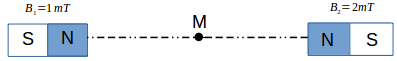
\includegraphics[scale=5, width=1\textwidth, center]{ex1}
%	\end{minipage}
	\begin{minipage}{0.60\textwidth}
		\item គេឲ្យរបាមេដែកចំនួន $3$ ដូចរូប ។ ចូរគូសវ៉ិចទ័រដែនម៉ាញេទិចទាំងបី រួចកំណត់ដែនម៉ាញេទិចផ្គួបត្រង់
		$M$ ។
	\end{minipage}
%	\begin{minipage}{0.40\textwidth}
%		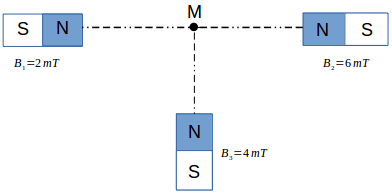
\includegraphics[width=1\textwidth, center]{ex2}
%	\end{minipage}
	\item បូប៊ីនមួយមានចំនួន $1000$ ស្ពៀ ដែលមានកាំ $R=2.5cm$ និងប្រវែង $50cm$ ។
	\begin{enumerate}[k]
		\item តើបូប៊ីននេះអាចចាត់ទុកជាសូលេណូអ៊ីតឬទេ?
		\item គេឲ្យចរន្ត $1A$ ឆ្លងកាត់ ចូរឲ្យលក្ខណៈសម្គាល់ដែនម៉ាញេទិចត្រង់ផ្ចិតរបស់វា ។ គេឲ្យ៖ $\mu_0=4\pi\times10^{-7}T\cdot m/A$
	\end{enumerate}
	\item បូប៊ីនមួយមានប្រវែង $1m$ និងមានអង្គត់ផ្ចិតខ្សែចម្លង $0.8mm$ ស្រោបដោយអ៊ីសូឡង់ដែលមានកម្រាស់ $0.1mm$ រុំជា ស្ពៀជាប់គ្នាៗលើស៊ីឡាំនោះ ។\\
	បើគេឲ្យចបឲរន្ត $1A$ ឆ្លងកាត់ ចូរគណនាអាំងឌុចស្យុងម៉ាញេទិច? គេឲ្យ៖ $\mu_0=4\pi\times10^{-7}T\cdot m/A$
	\item បូប៊ីនមួយមានប្រវែង $1m$  កើតឡើងដោយគេយកខ្សែរុំលើស៊ីឡាំងជា ស្ពៀជាប់ៗគ្នាឡាំង ចំនួន $3$ ជាន់ ហើយមានចរន្តឆ្លងកាត់ $10A$ ខ្សែចម្លងមានអង្គត់ផ្ចិត $1mm$ ។ គណនាអាំងឌុចស្យុងម៉ាញេទិច? គេឲ្យ៖ $\mu_0=4\pi\times10^{-7}T\cdot m/A$
	\item សូលេណូអ៊ីតមួយមានប្រវែង $50cm$ ហើយឆ្លងកាត់ដោយចរន្ត $I$ អាំងឌុចស្យុងម៉ាញេទិចត្រង់ផ្ចិតរបស់វាគឺ \\$B=12.56I\times10^{3}T$ ។
	\begin{enumerate}[k]
		\item រកចំនួនស្ពៀសរុប?
		\item រកចំនួនស្រទាប់ បើខ្សែចម្លងមានអង្គត់ផ្ចិត $1mm$? គេឲ្យ៖ $\mu_0=4\pi\times10^{-7}T\cdot m/A$
	\end{enumerate}
	\begin{center}
		\sffamily\color{black}
		សូមសំណាងល្អ!
	\end{center}\newpage
	\begin{center}
		\sffamily\color{black}
		\circled{០៤}\\
		មេរៀនទី​ ១ ដែន និងកម្លាំងម៉ាញេទិច(លំហាត់សុទ្ធ)
	\end{center}
	\begin{center}
		\sffamily\color{black}
		សូមសំណាងល្អ!
	\end{center}\newpage
\end{enumerate}
\end{document}